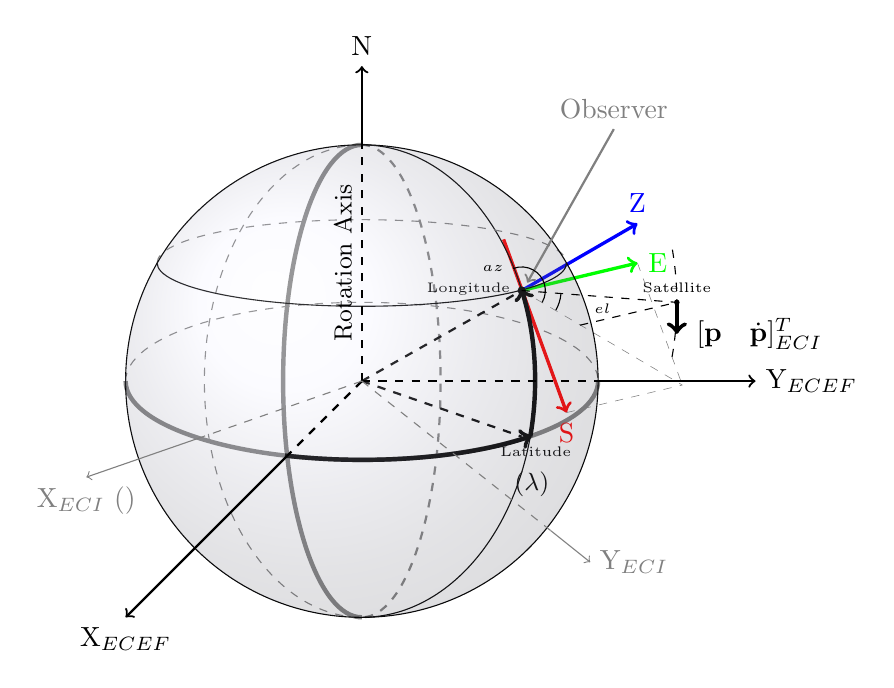
\begin{tikzpicture}
		
		\tikzset{
			partial ellipse/.style args={#1:#2:#3}{
				insert path={+ (#1:#3) arc (#1:#2:#3)}
			}
		}
		
		\setlength{\unitlength}{1cm};
		
		% Equator
		\draw[ultra thick, gray](-3,0) arc (180:360:3cm  and 1cm);
		\draw[dashed, gray] (-3,0) arc (180:0:3cm and 1cm);
		
		% 0 Meridian
		\draw[ultra thick, gray](0,3) arc (90:270:1cm and 3cm);
		\draw[dashed, thick, gray] (0,3) arc (90:-90:1cm and 3cm);
		
		% Radius
		\draw[dashed, thick](0,0) -- (2.03,1.15); 
		% Radius Projection 
		\draw[dashed, thick](0,0) -- (2.03,-0.705); 
		
		% SEZ Zenith
		\draw[very thick, blue, ->] (2.03,1.15) -- (3.5,2) node[above]{Z};
		% SEZ South
		\draw[very thick, red, ->] (1.8,1.8) -- (2.6,-0.4) node[below]{S};
		% SEZ East
		\draw[very thick, green, ->] (2.03,1.15) -- (3.5, 1.5) node[right]{E};
		% Point
		\fill (2.03,1.15) circle[radius=1.5pt];
		
		\draw[very thin, dashed, gray] (2.6,-0.4) -- (2.6 + 3.5 - 2.03, -0.4 + 1.5 - 1.15);
		\draw[very thin, dashed, gray] (3.5, 1.5) -- (3.5 + 2.6 - 2.03, 1.5 - 0.4 - 1.15);
		\draw[very thin, dashed, gray] (2.03,1.15) -- (3.5 + 2.6 - 2.03, 1.5 - 0.4 - 1.15);
		% SEZ South
		%\draw[thick, red] (2.03,1.15) -- (1.8, 1.8);
		
		% Observer Meridian
		\draw (0,3) arc (90:-90:2.2cm and 3cm);
		\draw[dashed, gray] (0,3) arc (90:270:2.cm and 3cm);
		\draw[ultra thick, ->] (0,0) [partial ellipse=-13.5:23:2.2cm and 3cm] node[left]{\tiny{Longitude}};     
		
		% Observer Latitude
		\draw (-2.6,1.5) arc (180:360:2.6cm  and 0.55cm);
		\draw[dashed, gray] (-2.6,1.5) arc (180:0:2.6cm and 0.55cm);
		\draw[ultra thick, ->] (0,0) [partial ellipse=251:316:3cm and 1cm]node[below, text width = 0.8cm, align = center]{\tiny{Latitude} \small{($\lambda$)}};
		
		% Sphere
		\draw (0,0) circle (3cm);
		\shade[ball color=blue!10!white,opacity=0.20] (0,0) circle (3cm);
		
		% North
		\draw[thick,dashed](0,0) -- (0,3) node[midway, above,sloped] {\small{Rotation Axis}}; \draw[thick,->](0,3) -- (0,4) node[above]{N};
		% Y ECEF
		\draw[dashed, thick](0,0) -- (3,0); \draw[thick,->](3,0) -- (5,0) 
		node[right]{Y$_{ECEF}$};
		% X ECEF
		\draw[dashed, thick](0,0) -- (-0.95,-0.95); \draw[thick,->](-0.95,-0.95) -- (-3,-3) node[below]{X$_{ECEF}$};
		
		% X ECI
		\draw[gray,dashed](0,0) -- (-2,-0.7); \draw[gray,->](-2,-0.7) -- (-3.5,-1.22) node[below]{X$_{ECI}$ (\aries)}; 
		% Y ECI
		\draw[gray,dashed](0,0) -- (2.4,-1.9); \draw[gray,->](2.4,-1.9) -- (2.9,-2.3) 
		node[right]{Y$_{ECI}$};
		
		% Observer arrow
		\draw[thick, gray, <-] (2.1, 1.25) -- (3.2,3.2) node[above]{Observer};
		
		% Satellite 
		\fill (4,1) circle[radius=1pt] node[above]{\tiny{Satellite}};
		
		\draw[thin, dashed] (2.03, 1.15) -- (4, 1);
		\draw[thin, dashed] (4 - 3.26 + 2.03, 1 - 1.44 + 1.15) -- (4,1);
		
		\draw (2.03,1.15) [partial ellipse=-30:-5:0.5cm] node[right= 15, below = -0.1]{\tiny{$el$}};
		
		\draw (2.03,1.15) [partial ellipse=-30:111:0.3cm] node[left]{\tiny{$az$}};
		
		% Satellite trajectory
		\draw[thin, dashed, -] (0,1) [partial ellipse=-10:10:4cm and 4cm];
		\draw[ultra thick, ->] (4, 1) -- (4,0.6) node[right = 3]{$[\textbf{p} \quad \dot{\textbf{p}}]^T_{ECI}$};
		
		\end{tikzpicture}